\begin{figure}[htbp]
\centering
\captionsetup{
  justification=raggedright,
  labelsep=none,
  singlelinecheck=false,
  labelformat=boldlabel,
}
\caption[Man and machine: active risk-return frontier.]{\footnotesize \textbf{: Man and machine: active risk-return frontier.} Annualized active return and risk for monthly rebalanced combinations holding $w$ in an ML Ensemble portfolio and $1-w$ in a human-manager benchmark. FUNDS\_MEAN and FUNDS\_Q75 are diversified fund portfolios; MED\_FUND and MED\_FUND\_Q75 report the median result across individual-fund combinations. In the two diversified panels the Information Ratio is the slope of a ray from the origin. In the two MED panels the coordinates are cross-fund medians of the components, so the slope is the median-component ratio and not the median of the fund-level Information Ratios reported in Table~\ref{combofront}. All returns are measured 15th-to-15th against IBOV. Squares, triangles and diamonds mark the pure manager, pure ML portfolio and maximum-IR combination. In the MED panels the $w=0$ square differs by ML scheme because months in which a fund does not report are held in that scheme's ML portfolio.}
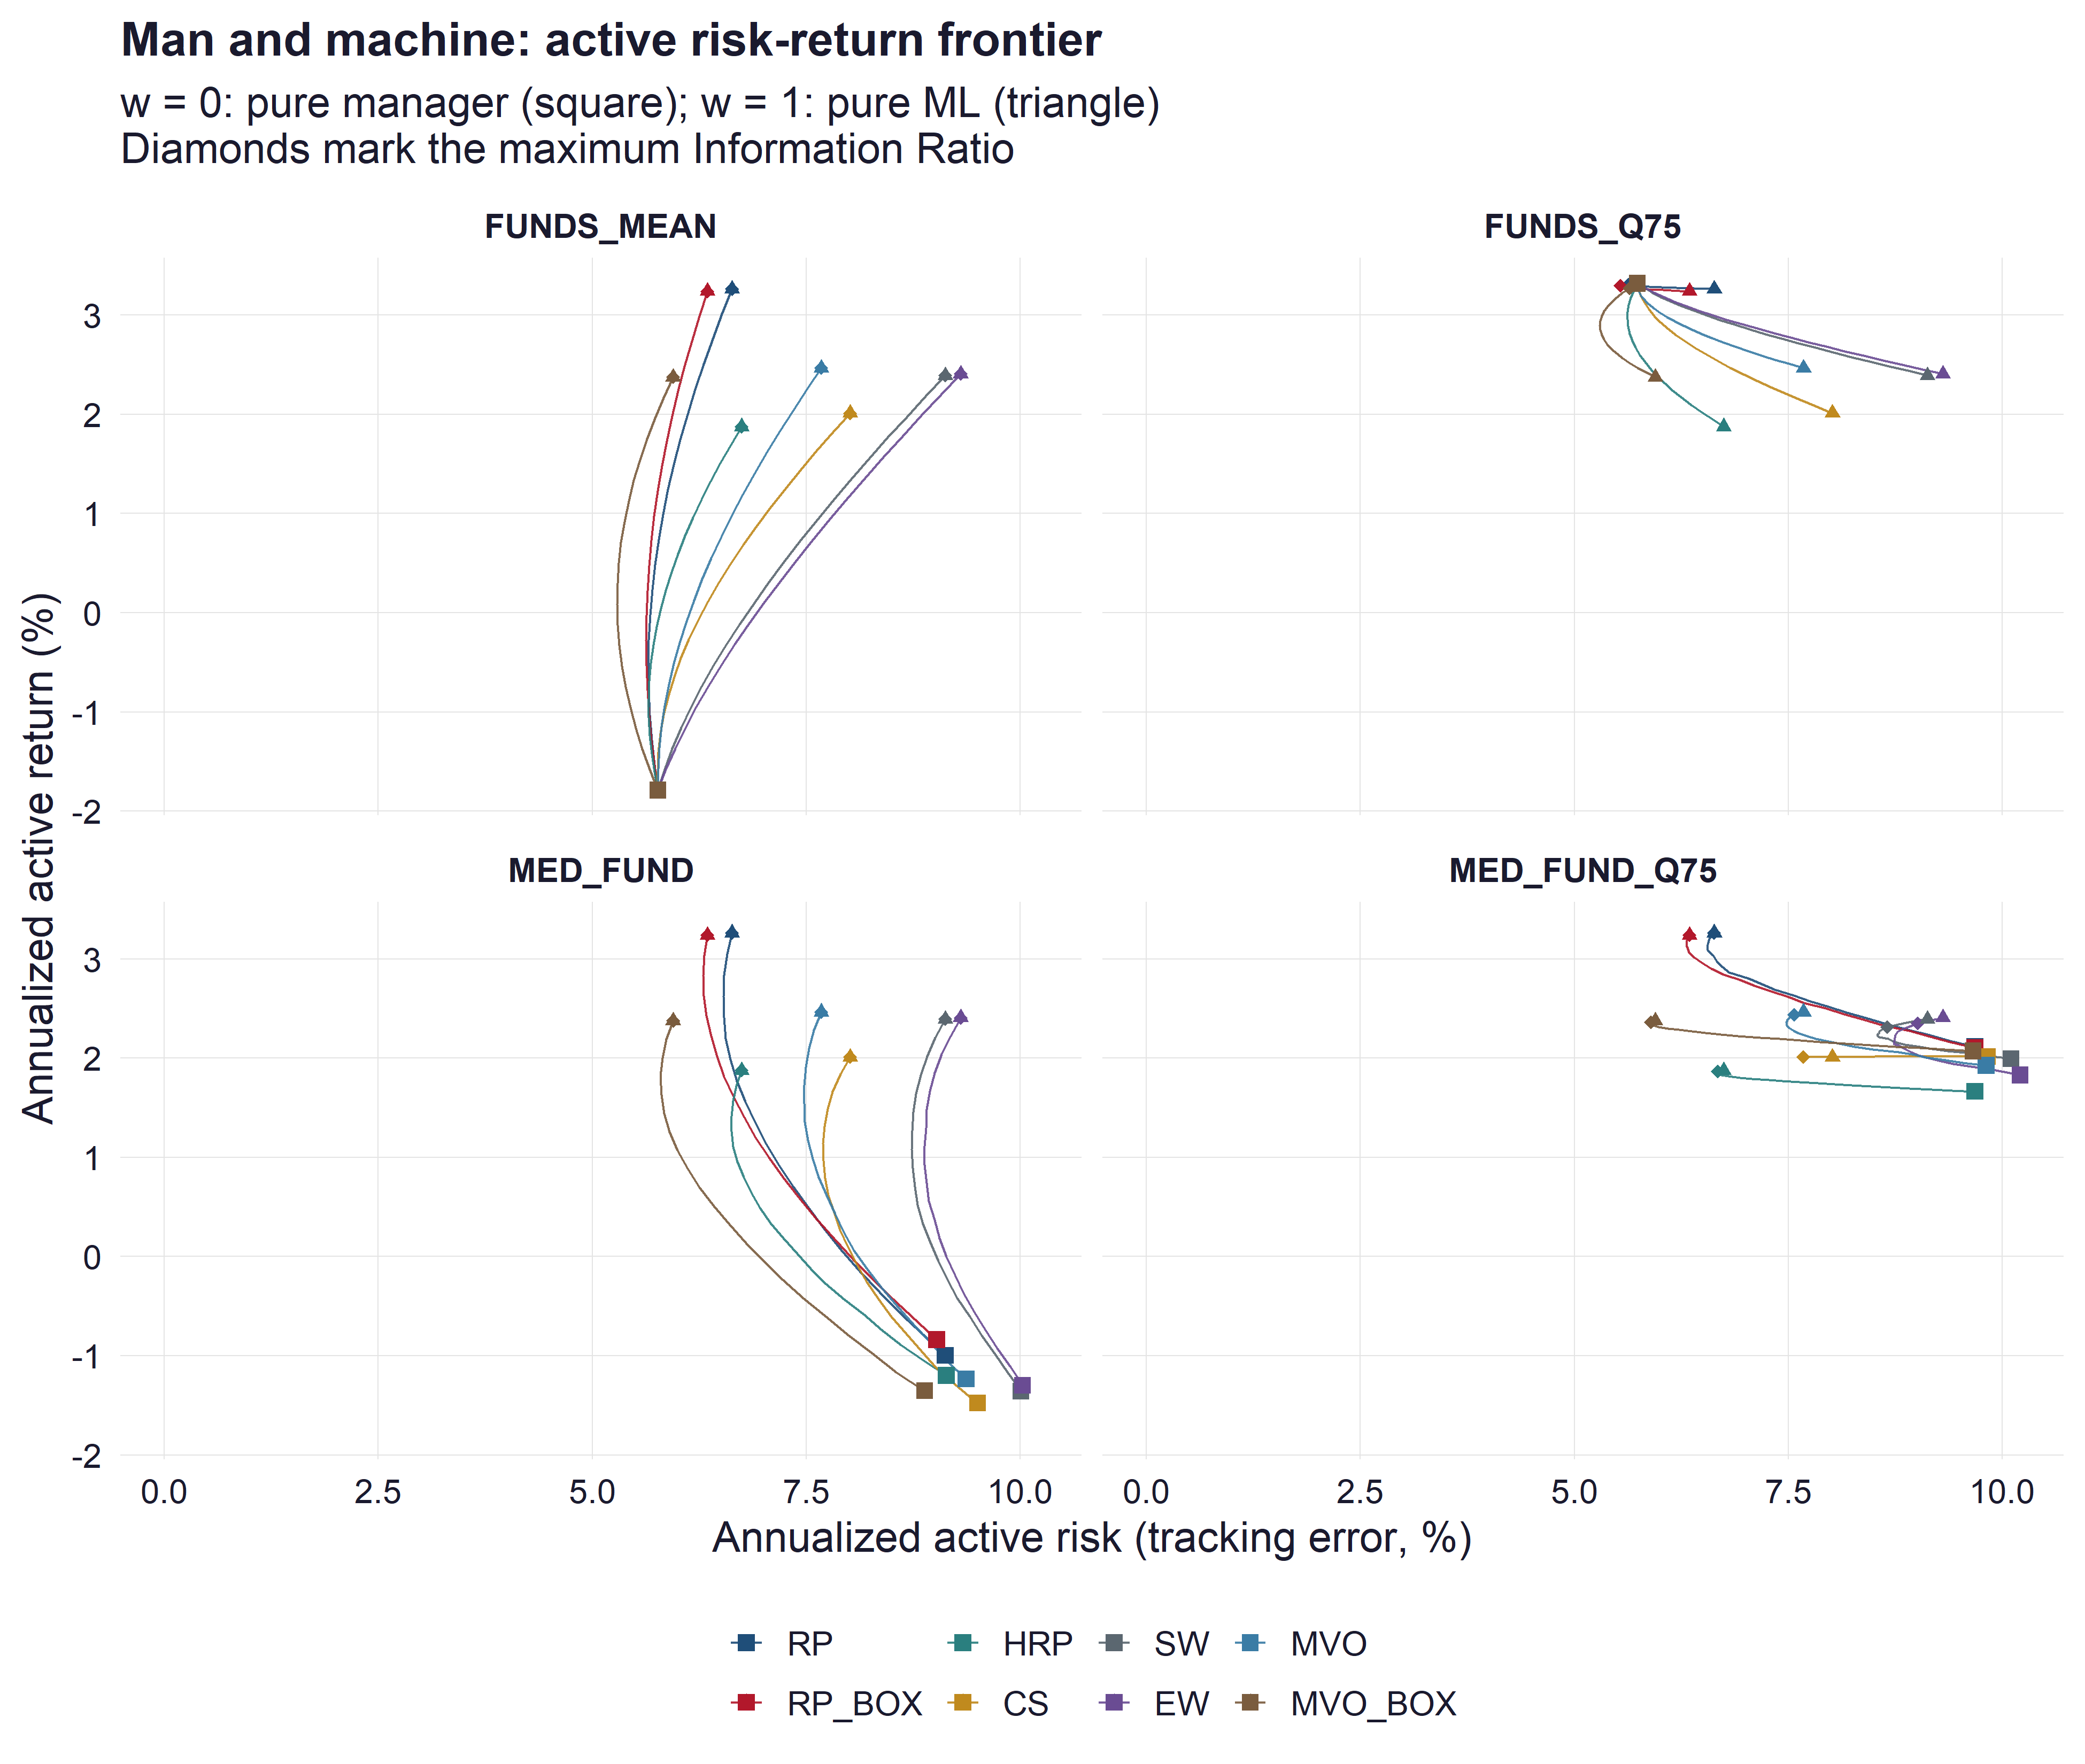
\includegraphics[width=\linewidth]{figures/combination_frontier.png}
\label{fig:combo_frontier}
\end{figure}
